\documentclass[aspectratio=169,hyperref={pdfpagelabels=false}]{beamer}
\usepackage{helvet}
\usepackage[english]{babel}
\usepackage{pgfplots}
\usepackage{pgf}
\pgfplotsset{compat=newest}
\usepackage{booktabs}
\usepackage[T1]{fontenc}
\usepackage[utf8]{inputenc}
\usepackage{lipsum}
\usepackage{tcolorbox}
\usepackage{xcolor}
\usepackage{listings}
\usepackage{microtype}
\usepackage{float}
\usepackage{siunitx}
\usepackage{multicol}
\usepackage{hyperref}
\usepackage{dsfont}
\usepackage{caption}
\usepackage{subcaption}

% DTU colours for diagrams
% You might want to make the front/back page background colour the first colour in the plot cycle list.
\pgfplotscreateplotcyclelist{DTU}{%
dtured,         fill=dtured,        \\%
blue,           fill=blue,          \\%
brightgreen,    fill=brightgreen    \\%
navyblue,       fill=navyblue       \\%
yellow,         fill=yellow         \\%
orange,         fill=orange         \\%
grey,           fill=grey           \\%
red,            fill=red            \\%
green,          fill=green          \\%
purple,         fill=purple         \\%
}

% Table of contents (TOC) and numbering of headings
\setcounter{tocdepth}{1}    % Depth of table of content: sub sections will not be included in table of contents
\setcounter{secnumdepth}{2} % Depth of section numbering: sub sub sections are not numbered



\newcommand{\setcolor}[1]{\def\chosencolor{#1}}
\newcommand{\setdepartment}[1]{\def\department{#1}}

\usetheme{DTU}
\setbeamersize{text margin left=22mm}
\def\insertframetitle{}

\newcommand{\inserttitlepage}{

    \begin{frame}[plain]{}
        \color{white}\maketitle    
    \end{frame}

    \setbeamercolor{background canvas}{bg = white}
}

\subtitle{Error Correction in Digital Systems}
\title{Project Introduction}
\author{Tjark Petersen}
\setcolor{orange}

\usepackage{multicol}
\usepackage{hyperref}
\usepackage{siunitx}
\usepackage{biblatex}

\addbibresource{ref.bib}

\newcommand{\sectionseperator}[1]{%

{%
\setbeamercolor{background canvas}{bg=\chosencolor}
\begin{frame}[plain]{}

        \usebeamercolor[fg]{title}

        \begin{center}
        \hspace{-3.6em}\vspace{-3.6em}{\usebeamerfont{title}\textbf{#1}\par}
        \end{center}

        
\end{frame}
}

}


\begin{document}
\inserttitlepage

\begin{frame}{Outline}

    \begin{itemize}
        \item Recap
        \item Lab 1
        \item Git
    \end{itemize}

\end{frame}


\sectionseperator{Recap}

\begin{frame}{The Fundamental Problem}
    % noisy channel
    \begin{itemize}
        \item Information is sent from $X$ to $Y$ via a \textit{noisy channel}
        \item The noisy channel randomly induces bit flips in the transmitted piece of information
        \item Solution: Adding redundant information in an encoder and using it in a decoder to restore the message
    \end{itemize}
    \begin{figure}
        \includegraphics[width=8cm]{../introduction_slides/fig/NoisyChannel.pdf}
    \end{figure}
\end{frame}

\begin{frame}{Project Plan}

    \begin{itemize}
        \item Start with some exercises on Hamming code and literature review on soft errors
        \item Implement part of an error correction capabable system in VHDL
        \item Write a technical report covering the theoretical background and your implementation using LaTeX
    \end{itemize}

    \begin{figure}
        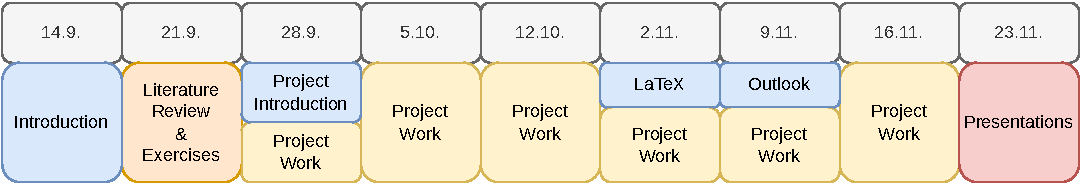
\includegraphics[width=\textwidth]{../introduction_slides/fig/CoursePlan.pdf}
    \end{figure}

\end{frame}

\begin{frame}{Lab 1}
    \begin{figure}
        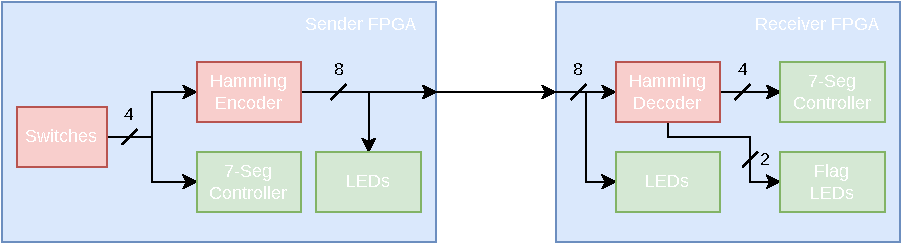
\includegraphics[width=\textwidth]{fig/Hamming_FPGA_system_block.pdf}
    \end{figure}
\end{frame}

\begin{frame}{Git}

    \begin{itemize}
        \item 
    \end{itemize}

\end{frame}



\end{document}